\begin{figure}[ht!]
    \centering

    \begin{subfigure}[t]{0.475\textwidth}
        \centering
        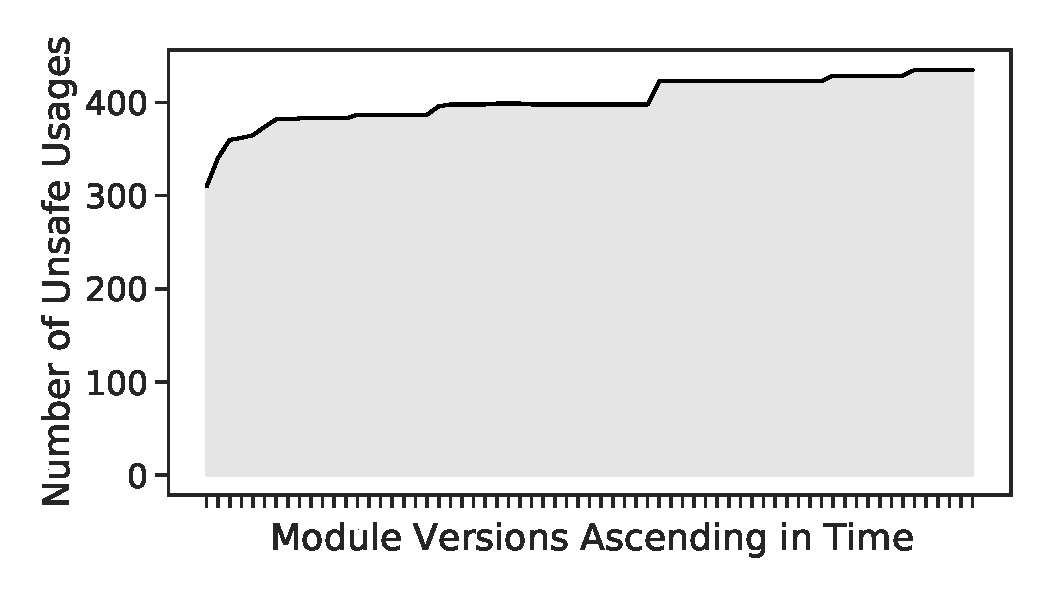
\includegraphics[width=\textwidth]{assets/plots/chapter4/unsafe-over-time-sys.pdf}
        \caption{\textit{golang.org/x/sys}}
        \label{subfig:unsafe-over-time:sys}
    \end{subfigure}
    \hfill
    \begin{subfigure}[t]{0.475\textwidth}
        \centering
        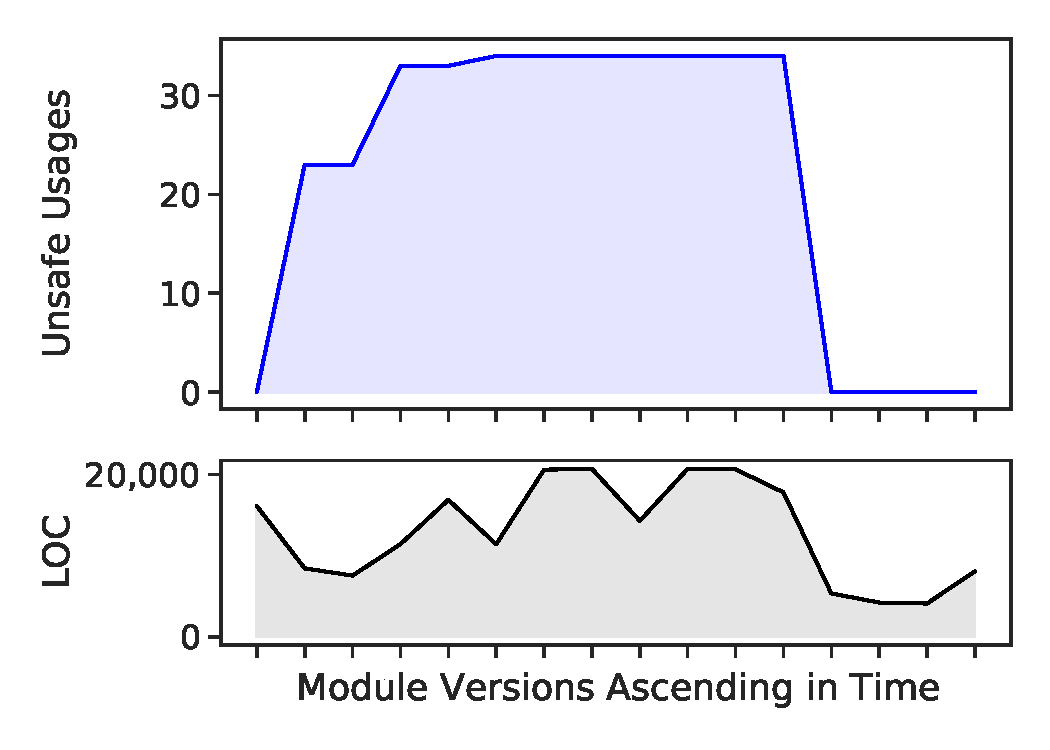
\includegraphics[width=\textwidth]{assets/plots/chapter4/unsafe-over-time-protobuf.pdf}
        \caption{\textit{github.com/golang/protobuf}}
        \label{subfig:unsafe-over-time:protobuf}
    \end{subfigure}
    \vskip\baselineskip
    \begin{subfigure}[t]{0.475\textwidth}
        \centering
        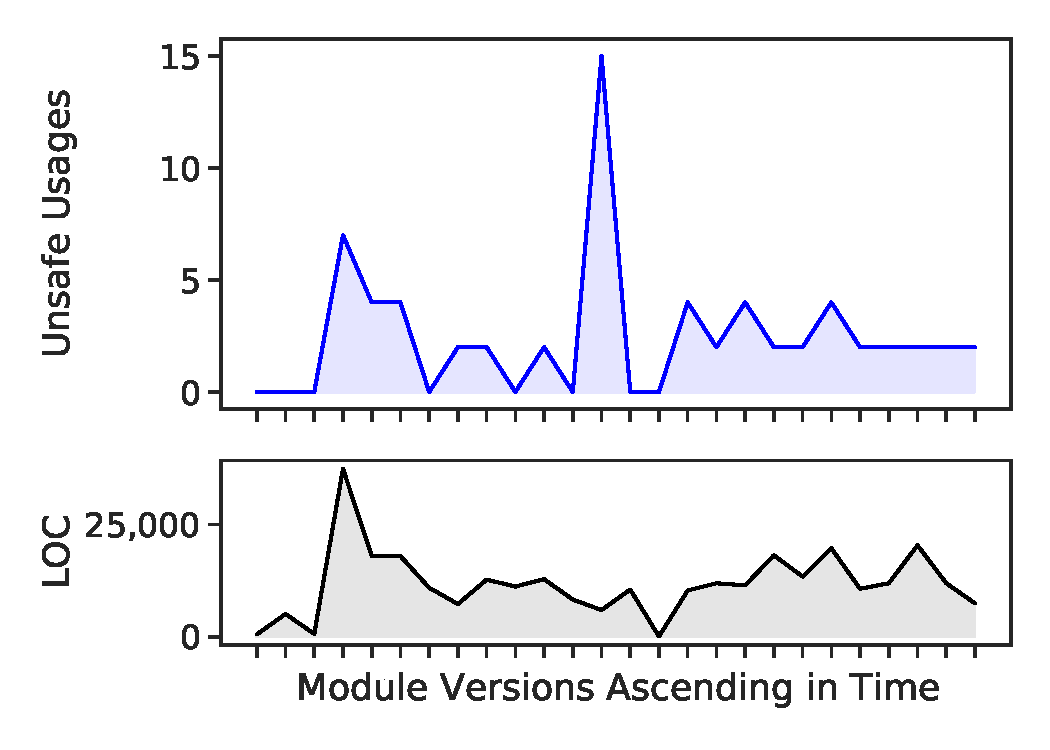
\includegraphics[width=\textwidth]{assets/plots/chapter4/unsafe-over-time-docker.pdf}
        \caption{\textit{github.com/docker/docker}}
        \label{subfig:unsafe-over-time:docker}
    \end{subfigure}
    \hfill
    \begin{subfigure}[t]{0.475\textwidth}
        \centering
        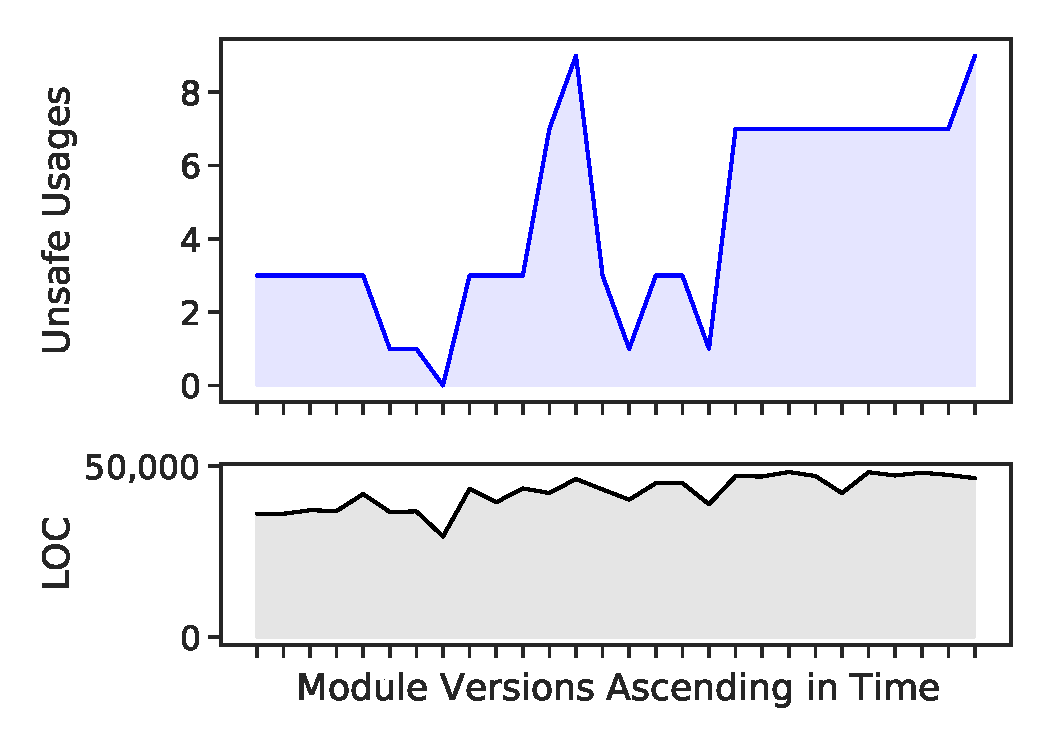
\includegraphics[width=\textwidth]{assets/plots/chapter4/unsafe-over-time-apimachinery.pdf}
        \caption{\textit{k8s.io/apimachinery}}
        \label{subfig:unsafe-over-time:apimachinery}
    \end{subfigure}

    \caption[Change of \unsafe{} usage in selected packages over time]
        {Change of \unsafe{} usage in selected packages over time.\newline\footnotesize~Each x tick represents one version. Note different scaling on y axes.}
    \label{fig:unsafe-over-time}
\end{figure}
